\chapter{Background material}

\section{The shortest path problem}
The shortest path problem is, as mentioned in the previous section, a well
known graph problem. Nevertheless I allow myself to brush up the readers
memory and define the problem.
\begin{defn}
    For a graph $G = (V, E)$ and a weight function $w : E \rightarrow
    \mathbb{R}$ mapping edges to edge weights.
    A path $p$ in $G$ is expressed by a sequence of vertices, where each
    vertex is adjacent with the next vertex in the sequence.
    \[
        p = \langle v_0, v_1, \dots ,v_i \rangle
    \]
    The weight of a path $w(p)$ is then given by the sum of the edge weights:
    \[
        w(p) = \sum\limits_{i=1}^k w(v_{i-1},v_{i})
    \]
    For two vertices $u,v \in V$. The \textbf{(shortest) distance}
    $\delta(u,v)$ from $u$ to $v$, is defined as:
    \[
        \delta(u,v) =
            \begin{cases}
                \text{min} \{ w(p): u \overset{p}{\leadsto} v \}
                & \text{if there exists a path from $u$ to $v$} \\
                \infty
                & \text{otherwise }
            \end{cases}
    \]
    A path $p$ from $u$ to $v$ is then a \textbf{shortest path} if and only if
    $w(p) = \delta(u,v)$.
\end{defn}
The shortest path problem described above may be referred to as \emph{single
pair shortest path}, but solutions to this problem requires the growth of
a shortest path tree from the source vertex, thus the computational
complexity of finding a shortest path between a vertex pair, is essentially the
same as finding the shortest path from the source vertex to all other vertices
in the graph.
Therefore the problem is often just referred to as \emph{single source
shortest path} or SSSP, even though in many cases only the distance
between a single vertex pair is of interest.

When constructing the approximate distance oracle data structure SSSP is
computed multiple times, thus in production environments an efficient SSSP
algorithm is needed. As mentioned in the previous section Thorup has presented
a SSSP algorithm for undirected graphs that offers a running time of $O(m)$
\cite{thorupsssp}. In the rest of this report I assume that SSSP is solved in
$O(m)$ unless mentioned otherwise.

\section{Shortest distances in large graphs}
Recent years - as we enter the age of big data - larger and larger graphs are
emerging. The World Wide Web, social networks, navigation service applications
and more has brought new attention to the shortest path problem, due the
increased space and time consumed by these new large graphs. Efficient
algorithms for the shortest path problem are important for two main reasons.

First of all, shortest path queries are the core product of many graph
applications, such as Google Maps, where a user requests a shortest path
between e.g Aarhus and Copenhagen.
Second, shortest path queries are used as building blocks in other algorithms
used to perform analytical tasks in graphs. E.g. centrality is calculated by
shortest path queries and include identifying the most influential persons in
a social network, key infrastructure nodes in the Internet, etc.
Also other measures, such as network diameter and betweenness, are based on
shortest path queries.

Well known algorithms such as Dijkstra and Bellman Ford solves the
problem of finding a shortest path, but a noticeable drawback of these
algorithms is that they are too slow for applications were fast results
are essential. The article "Toward a Distance Oracle for Billion-Node
Graphs"\cite{sp_billion_nodes} claim that for graphs of "web scale" it takes
hours for the Dijkstra algorithm to terminate.

As mentioned in the Introduction, a naive attempt to improve the query
time of shortest paths is to pre compute the distances. But the $O(n^2)$
space consumption makes this solution rather unrealistic. To put this into
perspective the largest graph for which I run experiments has 2 million
vertices.

\autoref{fig:matrixgrowth} shows the relationship between number of vertices
in the graph and the space consumption for the entries, I assume that an
integer takes up 32 bit of storage. To create a lookup table for the graph
with 2 million vertices I would have to store 30 terabyte of data, which seems
problematic. Graphs of this size is far from unusual today.

\begin{figure}[htbp]
    \centering
    \includegraphics[width=\textwidth]{matrixsize.pdf}
    \caption{Space consumption for $n\times n$ matrix, with 32 bit integers as entries}
    \label{fig:matrixgrowth}
\end{figure}

In general there is no doubt that the naive approach is unrealistic, as space
consumption rapidly exceeds the amount of disk space and memory available in
most computing environments.

The growth in applications using shortest paths and growth in the size of
large graphs, has led to increased research in data structures, which are
still able to answer shortest path queries extremely fast, but with improved
space complexity. Approximate distance oracles is a result of this research.

\chapter{Approximate distance oracles}
\label{sec:ado}
Thorup and Zwick presents a in the A\&C seminal paper "Approximate Distance
Oracles"\cite{tu}, the construction of a data structure that subsequently
can be used to answer shortest path queries extremely fast. The method can
be applied to connected undirected graphs with positive edge weights and is
feasible where approximated results are acceptable.

The paper sets forward two algorithms. The first one is the algorithm for
constructing the data structure called, we will refer to this algorithm as
\proc{propro}. The second one we call \proc{dist} and is used for querying
the data structured.

\proc{prepro} makes use of an integer $k$, that lets one weigh the precision
(maximum stretch) of the estimated distances versus space and time consumption.

An estimate of the shortest distance, denoted $\hat{\delta}$, from vertex $u$
to vertex $v$ is said to be of stretch $t$ if and only if
\begin{equation}
    \delta(u,v) \leq \hat{\delta}(u,v) \leq t \cdot \delta(u,v)
    \label{eq:stretchinterval}
\end{equation}
The properties of the data structure and the relationship between $k$ and the
stretch is formulated in the theorem below\footnote{\cite{tu}, Theorem 1.1}.
\begin{thm}
    Let $G=(V,E)$ be a weighed undirected graph with nonnegative edge weights
    with $|V|=n, |E|=m$. Let $k \geq 1$ be an integer. Then, the graph $G$
    can be preprocessed in $O(kmn^{1/k})$ expected time, producing a data
    structure of $O(kn^{1+1/k}$, such that subsequent distance queries can
    be answered, approximately, in $O(k)$ time. The stretch of the produced
    estimates is at most $2k-1$. Paths no longer than the estimates returned
    can be produced in constant time.\footnote{In this report I do not care
    for the actual path found by the algorithm, only for the distance of
    the path, and thus the last sentence of Threorem\autoref{thm:ado_prop} is
    only present for completion.}
    \label{thm:ado_prop}
\end{thm}
By choosing $k=1$ we get a solution similar to computing all distances
and saving the results, that is $O(mn)$ preprocessing time, $O(n^2)$ space
consumption and a worst case stretch of $1$. When $k=2$ we get a
preprocessing time of $O(mn^{1/2})$, space consumption is $O(n^{3/2})$ and
the stretch is now $3$. This trend continues until $k \gets log(n)$. For $k$
greater than $log(n)$ space and time consumption will not improve as the
functions for space and time complexity finds their local minimum where $k
\gets log(n)$.

The essence of approximate distance oracles is to make use of a collection of
induced trees that form a tree cover of the whole graph. The reduced space
consumption is achieved, because each vertex is only contained in a small
number of the trees. The construction algorithm assures that for each vertex
pair there exists a tree with a small-stretched path between the two vertices.

From the trees the article derive a bunch $B(v) | v \in V$ for each vertex in
the graph. A bunch is a collection of vertices for which the shortest distance
is known. In practice a bunch $B(v)$ for a vertex $v$ is a hash map with a
vertex $u$ as key and the distance $\delta(u,v)$ as value.

Besides bunches, the algorithms make use what is referred to as witnesses.
A witness to a vertex $v$ is denoted as $p_{i}{v}$, where $i$ refers a
specific set ($A_{i}$) of vertices in the graph. The witness for a specific
vertex $v$ and set $A_{i}$ is a tuple containing a vertex $w$ and a distance
$\delta(v,w)$. The witness is the vertex in the set $A_{i}$, with the shortest
distance to $v$.

A graphic representation of bunches and witnesses for $u$ and $v$ is depicted
in \autoref{fig:bunches}.
\begin{figure}[htbp]
    \centering
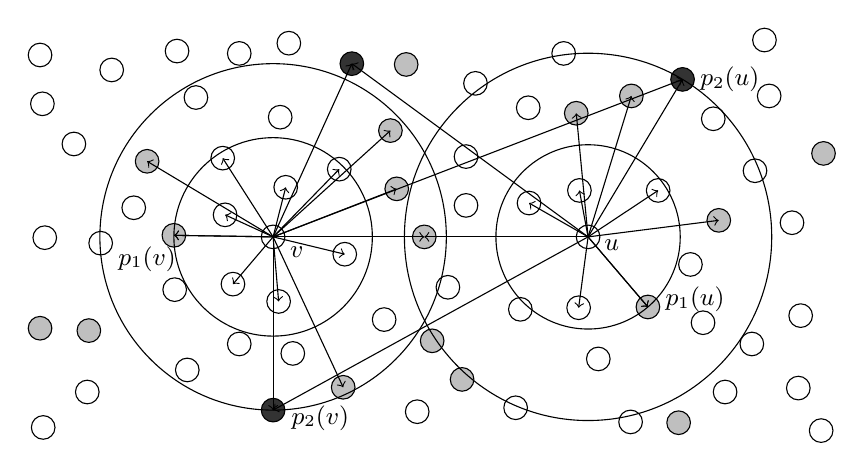
\begin{tikzpicture}
    \filldraw[fill=white, draw=black] (0.04,4.81) circle [radius=1.50mm];
    \filldraw[fill=white, draw=black] (0.07,4.19) circle [radius=1.50mm];
    \filldraw[fill=white, draw=black] (0.08,0.08) circle [radius=1.50mm];
    \filldraw[fill=white, draw=black] (0.1,2.49) circle [radius=1.50mm];
    \filldraw[fill=white, draw=black] (0.47,3.68) circle [radius=1.50mm];
    \filldraw[fill=white, draw=black] (0.64,0.53) circle [radius=1.50mm];
    \filldraw[fill=white, draw=black] (0.81,2.42) circle [radius=1.50mm];
    \filldraw[fill=white, draw=black] (0.95,4.62) circle [radius=1.50mm];
    \filldraw[fill=white, draw=black] (1.23,2.87) circle [radius=1.50mm];
    \filldraw[fill=white, draw=black] (1.75,1.83) circle [radius=1.50mm];
    \filldraw[fill=white, draw=black] (1.78,4.86) circle [radius=1.50mm];
    \filldraw[fill=white, draw=black] (1.91,0.81) circle [radius=1.50mm];
    \filldraw[fill=white, draw=black] (2.02,4.27) circle [radius=1.50mm];
    \filldraw[fill=white, draw=black] (2.36,3.5) circle [radius=1.50mm];
    \filldraw[fill=white, draw=black] (2.39,2.78) circle [radius=1.50mm];
    \filldraw[fill=white, draw=black] (2.49,1.9) circle [radius=1.50mm];
    \filldraw[fill=white, draw=black] (2.57,1.14) circle [radius=1.50mm];
    \filldraw[fill=white, draw=black] (2.57,4.83) circle [radius=1.50mm];
    \filldraw[fill=white, draw=black] (3.07,1.68) circle [radius=1.50mm];
    \filldraw[fill=white, draw=black] (3.09,4.02) circle [radius=1.50mm];
    \filldraw[fill=white, draw=black] (3.16,3.13) circle [radius=1.50mm];
    \filldraw[fill=white, draw=black] (3.2,4.96) circle [radius=1.50mm];
    \filldraw[fill=white, draw=black] (3.25,1.02) circle [radius=1.50mm];
    \filldraw[fill=white, draw=black] (3.84,3.36) circle [radius=1.50mm];
    \filldraw[fill=white, draw=black] (3.91,2.28) circle [radius=1.50mm];
    \filldraw[fill=white, draw=black] (4.41,1.45) circle [radius=1.50mm];
    \filldraw[fill=white, draw=black] (4.83,0.28) circle [radius=1.50mm];
    \filldraw[fill=white, draw=black] (5.22,1.86) circle [radius=1.50mm];
    \filldraw[fill=white, draw=black] (5.45,2.9) circle [radius=1.50mm];
    \filldraw[fill=white, draw=black] (5.45,3.52) circle [radius=1.50mm];
    \filldraw[fill=white, draw=black] (5.57,4.45) circle [radius=1.50mm];
    \filldraw[fill=white, draw=black] (6.08,0.33) circle [radius=1.50mm];
    \filldraw[fill=white, draw=black] (6.14,1.58) circle [radius=1.50mm];
    \filldraw[fill=white, draw=black] (6.24,4.14) circle [radius=1.50mm];
    \filldraw[fill=white, draw=black] (6.25,2.93) circle [radius=1.50mm];
    \filldraw[fill=white, draw=black] (6.69,4.83) circle [radius=1.50mm];
    \filldraw[fill=white, draw=black] (6.88,1.6) circle [radius=1.50mm];
    \filldraw[fill=white, draw=black] (6.89,3.09) circle [radius=1.50mm];
    \filldraw[fill=white, draw=black] (7.13,0.95) circle [radius=1.50mm];
    \filldraw[fill=white, draw=black] (7.54,0.15) circle [radius=1.50mm];
    \filldraw[fill=white, draw=black] (7.89,3.09) circle [radius=1.50mm];
    \filldraw[fill=white, draw=black] (8.3,2.15) circle [radius=1.50mm];
    \filldraw[fill=white, draw=black] (8.46,1.41) circle [radius=1.50mm];
    \filldraw[fill=white, draw=black] (8.59,4.0) circle [radius=1.50mm];
    \filldraw[fill=white, draw=black] (8.74,0.53) circle [radius=1.50mm];
    \filldraw[fill=white, draw=black] (9.08,1.14) circle [radius=1.50mm];
    \filldraw[fill=white, draw=black] (9.12,3.34) circle [radius=1.50mm];
    \filldraw[fill=white, draw=black] (9.24,5.0) circle [radius=1.50mm];
    \filldraw[fill=white, draw=black] (9.3,4.29) circle [radius=1.50mm];
    \filldraw[fill=white, draw=black] (9.59,2.68) circle [radius=1.50mm];
    \filldraw[fill=white, draw=black] (9.67,0.58) circle [radius=1.50mm];
    \filldraw[fill=white, draw=black] (9.7,1.5) circle [radius=1.50mm];
    \filldraw[fill=white, draw=black] (9.96,0.04) circle [radius=1.50mm];
    \filldraw[fill=gray!50, draw=black] (0.04,1.34) circle [radius=1.50mm];
    \filldraw[fill=gray!50, draw=black] (0.66,1.31) circle [radius=1.50mm];
    \filldraw[fill=gray!50, draw=black] (1.4,3.46) circle [radius=1.50mm];
    \filldraw[fill=gray!50, draw=black] (1.74,2.52) circle [radius=1.50mm];
    \filldraw[fill=gray!50, draw=black] (3.89,0.59) circle [radius=1.50mm];
    \filldraw[fill=gray!50, draw=black] (4.49,3.85) circle [radius=1.50mm];
    \filldraw[fill=gray!50, draw=black] (4.57,3.11) circle [radius=1.50mm];
    \filldraw[fill=gray!50, draw=black] (4.69,4.69) circle [radius=1.50mm];
    \filldraw[fill=gray!50, draw=black] (4.92,2.5) circle [radius=1.50mm];
    \filldraw[fill=gray!50, draw=black] (5.02,1.18) circle [radius=1.50mm];
    \filldraw[fill=gray!50, draw=black] (5.4,0.69) circle [radius=1.50mm];
    \filldraw[fill=gray!50, draw=black] (6.85,4.07) circle [radius=1.50mm];
    \filldraw[fill=gray!50, draw=black] (7.55,4.29) circle [radius=1.50mm];
    \filldraw[fill=gray!50, draw=black] (7.76,1.61) circle [radius=1.50mm];
    \filldraw[fill=gray!50, draw=black] (8.15,0.14) circle [radius=1.50mm];
    \filldraw[fill=gray!50, draw=black] (8.66,2.71) circle [radius=1.50mm];
    \filldraw[fill=gray!50, draw=black] (9.99,3.56) circle [radius=1.50mm];
    \filldraw[fill=black!80, draw=black] (3,0.3) circle [radius=1.50mm];
    \filldraw[fill=black!80, draw=black] (4,4.7) circle [radius=1.50mm];
    \filldraw[fill=black!80, draw=black] (8.2,4.5) circle [radius=1.50mm];
    \filldraw[fill=white, draw=black] (3,2.5) circle [radius=1.50mm];
    \node at (3.3,2.3) {\small$v$};
    \draw(3,2.5) circle [radius=1.26015872016cm];
    \node at (1.4,2.22) {\small$p_1(v)$};
    \draw [->] (3,2.5) -- (1.74,2.52);
    \draw [->] (3,2.5) -- (3.07,1.68);
    \draw [->] (3,2.5) -- (2.36,3.5);
    \draw [->] (3,2.5) -- (2.39,2.78);
    \draw [->] (3,2.5) -- (3.91,2.28);
    \draw [->] (3,2.5) -- (2.49,1.9);
    \draw [->] (3,2.5) -- (3.16,3.13);
    \draw [->] (3,2.5) -- (3.84,3.36);
    \draw(3,2.5) circle [radius=2.2cm];
    \node at (3.6,0.2) {\small$p_2(v)$};
    \draw [->] (3,2.5) -- (1.74,2.52);
    \draw [->] (3,2.5) -- (3.89,0.59);
    \draw [->] (3,2.5) -- (4.49,3.85);
    \draw [->] (3,2.5) -- (1.4,3.46);
    \draw [->] (3,2.5) -- (4.57,3.11);
    \draw [->] (3,2.5) -- (4.92,2.5);
    \draw [->] (3,2.5) -- (4,4.7);
    \draw [->] (3,2.5) -- (3,0.3);
    \draw [->] (3,2.5) -- (8.2,4.5);
    \filldraw[fill=white, draw=black] (7,2.5) circle [radius=1.50mm];
    \node at (7.3,2.4) {\small$u$};
    \draw(7,2.5) circle [radius=1.17034183041cm];
    \node at (8.36,1.71) {\small$p_1(u)$};
    \draw [->] (7,2.5) -- (7.76,1.61);
    \draw [->] (7,2.5) -- (7.89,3.09);
    \draw [->] (7,2.5) -- (6.89,3.09);
    \draw [->] (7,2.5) -- (6.25,2.93);
    \draw [->] (7,2.5) -- (6.88,1.6);
    \draw(7,2.5) circle [radius=2.33238075794cm];
    \node at (8.8,4.5) {\small$p_2(u)$};
    \draw [->] (7,2.5) -- (7.55,4.29);
    \draw [->] (7,2.5) -- (7.76,1.61);
    \draw [->] (7,2.5) -- (6.85,4.07);
    \draw [->] (7,2.5) -- (4.92,2.5);
    \draw [->] (7,2.5) -- (8.66,2.71);
    \draw [->] (7,2.5) -- (4,4.7);
    \draw [->] (7,2.5) -- (3,0.3);
    \draw [->] (7,2.5) -- (8.2,4.5);
\end{tikzpicture}
\caption{Bunches and witnesses for $u$ and $v$}
\label{fig:bunches}
\end{figure}

With these basic concepts loosely introduced, I will introduce the algorithm
for constructing the data structure and discuss it in more detail.

\section{Creating the data structure}
\label{sec:ado:creation}
Pseudo code for the preprocessing algorithm \proc{prepro} is given in
\autoref{pseudo:prepro}. It receives as input an undirected graph $G(V,E)$ and
returns bunches and witnesses.

\begin{figure}[htbp]
\begin{codebox}
    \Procname{$\proc{prepro}_{k}(V, E)$}
    \li $A_{0}\gets V$; $A_{k}\gets \emptyset$ 
    \li \For $i \gets 1$ \To $k-1$
    \li \Do
            let $A_{i}$ contain each element of $A_{i-1}$,
    \zi     independently, with probability $n^{-1/k}$.
        \End

    \li \For $v \in V$ 
    \li \Do
            $\delta(A_{k}, v) \gets \infty$ 
        \End

    \li \For $i \gets k-1 \Downto 0$ 
    \li \Do

            \For every $v \in V$ 
    \li     \Do
                compute $\delta(A_{i},v)$ and find $p_{i}(v) \in A_{i}$ 
    \zi         such that $\delta(p_{i}(v),v) \isequal \delta(A_{i},v)$
    \zi     \Comment **
            \End

    \li     \For every $w \in A_{i} - A_{i+1}  $ 
    \li     \Do
                grow shortest path tree $T(w)$ from $w$
    \zi         spanning $C(w) = \{v \in V | \delta(w,v) < \delta(A_{i+1},v) \}$
            \End
        \End

    \li \For every $v \in V$ 
    \li \Do
        let $B(v) \gets \{w \in V | v \in C(w) \}$
        \End
    \li \Return $B(\dots)$, $p(\dots)$
\end{codebox}
\caption{The preprocessing algorithm}
\label{pseudo:prepro}
\end{figure}
Looking at \autoref{fig:bunches} one can see that the circles representing the
vertices have different colors, to denote the vertices is part different sets.

When constructing the data structure the algorithm start by creating the
sets $A_0$ to $A_{k}$ $A_0 \gets V$ and $A_{k} \gets \emptyset$, each set in
between is constructed by letting $A_i$ contain each element of $A_{i-1}$,
independently with probability $n^{-1/k}$. Note, that these sets are not
disjoint and are constructed in such a way that $A_{0} \supseteq A_1 \supseteq
\cdots \supseteq A_{k-1} \supseteq A_{k}$. We refer to these sets $A_i$ as
\emph{$i$-centers}.

When all $i$-centers are constructed the algorithm enters a for-loop
with $k$ iterations. For the $i$'th iteration, the algorithm determines the
distance to the $i$'th $i$-center $\delta(A_i , v)$ for every $v \in V$, that is
$\delta(A_i , v) = \textrm{min}\{\delta(w,v)\,|\,w \in A_i\}$. Also a witness 
$p_{i}(v)$ is found such that $\delta(p_{i}(v),v) = \delta(A_i , v)$.

This is done by adding a new vertex $h$ to the graph $G=(V,E)$ and for each
vertex in the $i$-center $w \in A_i$, adding an edge with weight $0$ between
$h$ and $w$. The distances are found in $O(m)$ by using Thorups SSSP algorithm,
and the returned shortest path tree is used to determine the witnesses for
each $v \in V$. $h$ is removed from the graph after the SSSP completes.

Still in the $i$'th iteration, the algorithm constructs clusters $C(w)$ around
each $i$-center $w \in A_i - A_{i+1}$. The clusters are constructed such that
$C(w) = {v \in V \,|\, \delta(w,v) < \delta(A_{i+1}, v)}$, that is the cluster
to $w$ holds all the vertices $v \in V$ which are closer to $w$, than to
the nearest $(i+1)$-center. As $\delta(A_k, v) = \infty$ for every $v \in
V$, the clusters generated for $w \in A_{k-1}-A_{k}$ (remember $A_{k-1}
= A_{k-1}-A_{k}$ because $A_{k}=\emptyset$) will span the whole graph.
\autoref{fig:cluster} depicts the cluster construction.
\begin{figure}[htbp]
    \centering
    \includegraphics[width=0.8\textwidth]{clusterconstruct.png}
    \caption{Clusters constructed by the modified SSSP algorithm, the figure
             is taken directly from the article\cite{tu}}.
    \label{fig:cluster}
\end{figure}
The clusters are computed by running a modified SSSP algorithm. Due to the
complexity of Thorups SSSP algorithm I will illustrate the modification
on Dijkstra. My implementation used for experiments in later sections also
uses a modified Dijkstra to compute the clusters, so the code is in
agreement with this modification on Dijkstra.

The modification to Dijkstra is in the relaxation step. A normal Dijkstra
relaxes as such
\begin{codebox}
    \Procname{$\proc{relax}(u, v)$}
    \li \If $d(v) > d(u) + \ell(u,v)$
    \li     \Do
            $d(v) = d(u) + \ell(u,v)$
            \End
\end{codebox}
Thorup and Zwick changes this step, so that clusters now are constructed
instead by only including the vertices that are closer to $w$ than to the
$(i+1)$-center.
\begin{codebox}
    \Procname{$\proc{relax\_modified}(u, v)$}
    \li \If $\delta(A_{i+1},v) > d(u) + \ell(u,v)$
    \li     \Do
            $d(v) = d(u) + \ell(u,v)$
            \End
\end{codebox}
After all clusters are constructed the algorithm creates the bunches, as
defined by the algorithm $w \in B(v)$ if and only $v \in C(w)$. The clusters
and the bunches hold the exact same information. The benefit of the bunches
is that the information used by \proc{dist } to find a shortest path can be
stored with the vertex, and thus bunches allow for distance labeling.

The relationship between clusters and bunches is also clear if one takes a
closer look at \autoref{fig:cluster}. E.g if I take a white vertex, that is
a vertex only in $A_0-A_1$, I see that the connected gray vertex should be
part of the bunch, because the gray vertex is closer to the white than to the
black vertex, that is $w \in A_1 - A_2 \,|\, \delta(w,v) < \delta(A_2,v)$.

After the construction of bunches the algorithm terminates and returns the
bunches and witnesses.

\section{Answering shortest distance queries}
The algorithm, \autoref{pseudo:dist}, used to produce estimates from the
constructed data structure is straight forward. The algorithm works by
checking if the vertex $w$ is in the bunch of $v$. If that is not the case $u$
and $v$ are swapped, $i$ is incremented and $w$ is set to $u$'s witness of the
incremented $i$-center. Because $A_{k-1} \in B(v)$ the algorithm will always
terminate.

When $w \in B(v)$ the algorithm returns the estimated distance by reading
$\delta(w,u)$ from the witnesses. The distance $\delta(w,v)$ is read directly
from the bunch $B(v)$.

\begin{figure}[htbp]
\begin{codebox}
    \Procname{$\proc{dist}_{k}(u, v)$}
    \li $w \gets u$
    \li $i \gets 0$ 
    \li \While $w \notin B(v)$
    \li     \Do
                $i \gets i+1$
    \li         $(u,v) \gets (v,u)$
    \li         $w \gets p_{i}(u)$
            \End
    \li \Return $\delta(w,u) + \delta(w,v)$
\end{codebox}
\caption{The distance query algorithm}
\label{pseudo:dist}
\end{figure}

\section{Average stretch of estimates}
From \autoref{eq:stretchinterval} one can see approximate distance oracles
produces results with a stretch guarantee $t$. That is a worst-case multiplicative
factor increase of the distance between a pair of vertices. But this worst case
guarantee may differ substantially from the average multiplicative factor on the
produced distances. For a shortest path query the actual stretch on the distance is
denoted $s$ and is the fraction of the estimated shortest distance over
the exact shortest distance.
\begin{equation}
    s(u,v) = \frac{\hat{\delta}(u,v)}{\delta(u,v)}
\end{equation}
Thus, there will also exist an average actual stretch for a given data structure
\begin{equation}
    \bar{s} = \frac{\sum\limits_{(u,v) \in V \times V} s(u,v) }{|V|^2}
\end{equation}
The article by Thorup and Zwick\cite{tu} does not mention the actual stretch
of the estimates $s$ or the average actual stretch $\bar{s}$. It is my goal to
determine $\bar{s}$ for the graphs used in my experiments, and try to indicate
what values to expect for the classes of graphs used in my experiments.
